\documentclass[a4paper, 12pt]{article}
\usepackage{graphicx}

\renewcommand{\thesubsection}{\thesection.\alph{subsection}}


\usepackage{xparse}
\ExplSyntaxOn
\NewDocumentCommand{\Rowvec}{ O{,} m }
{
	\vector_main:nnnn { p } { & } { #1 } { #2 }
}
\NewDocumentCommand{\Colvec}{ O{,} m }
{
	\vector_main:nnnn { p } { \\ } { #1 } { #2 }
}

\seq_new:N \l__vector_arg_seq
\cs_new_protected:Npn \vector_main:nnnn #1 #2 #3 #4
{
	\seq_set_split:Nnn \l__vector_arg_seq { #3 } { #4 }
	\begin{#1matrix}
		\seq_use:Nnnn \l__vector_arg_seq { #2 } { #2 } { #2 }
	\end{#1matrix}
}
\ExplSyntaxOff

\usepackage{enumitem}
\usepackage{t1enc}
\usepackage[utf8]{inputenc}
\usepackage[magyar]{babel}

% a szép matematikai szimbólumokért
\usepackage{amssymb}
\usepackage{amsmath}
\usepackage{nccmath}
\usepackage{siunitx}

\usepackage{listings}
\lstset{language=Python}

\usepackage{subcaption}
\usepackage[justification=centering]{caption}

% ha táblázatban szeretnénk egyesített sorokat is
\usepackage{multirow}

% horizontal line
\usepackage{hhline}

% eps formátumú ábrák --> pdflatex fordításhoz!!
\usepackage{epsfig}

% egyenletekhez, pl mátrixok írására
\usepackage{array}

% ha betűszíneket is szeretnénk használni
\usepackage{color}

% Margók egyéni beállításai
\usepackage{anysize}
\marginsize{1.64cm}{1.64cm}{1.2cm}{2.4cm} %\left right top bottom

% vakszöveg
\usepackage{lipsum}
\usepackage{blindtext}

% A HIVATKOZÁSOKHOZ HASZNÁLT CSOMAGOK. RÉSZLETESEBBEN LD: google -> latex bibtex
\usepackage[numbers, square, comma, sort&compress]{natbib}
%\usepackage[format=hang,labelsep=period]{caption}

\usepackage[unicode]{hyperref}   % ezzel a hivatkozások linkké válnak
\usepackage{bookmark}
\hypersetup{bookmarksopen={true}}
\hypersetup{bookmarksopenlevel={2}}
\hypersetup{bookmarksnumbered={true}}
\hypersetup{
	colorlinks,%
	citecolor=red,%
	filecolor=black,%                                                                                                                                               
	linkcolor=blue,%
	urlcolor=green
}
\numberwithin{equation}{section}          % ezekkel tudod beállítani, hogy milyen felbontásig menjen a hivatkozás
\numberwithin{figure}{subsection}
%\numberwithin{table}{section}          % ha kikommenteled, akkor csak simán számozva lesz.

%%%%%%%%%%%%%%%% Néhány dolog a fancy kinézethez

\frenchspacing
\setlength{\parskip}{2ex}
\setlength{\headsep}{1cm}
\setlength{\headheight}{4pt}

% fej- es lábléc
\usepackage{fancyhdr}
\usepackage{fancyref}
\usepackage{fancyvrb}
\pagestyle{fancy}

\renewcommand{\headrulewidth}{2pt}
\renewcommand{\footrulewidth}{0pt}


\fancyhf{}
\fancyhead[LO]{{ \nouppercase{\rightmark}} }

\cfoot{--~\thepage~--}

%%%%%%%%%%%%%%%%%%%%%%%%%%%


%%%%%%%%%%%%%%%%%%%%%%%%%%%%%%%%%%%%%%%%%%%%%%%%%%%%%%%%%%%%%%%%%%%%%%%%%%%%

\begin{document}

% Címoldalt lehet egyszerűen a \maketitle paranccsal is. Ha kissé részletesebb
% címre van szükség, azt lehet így is, kézzel megadva mindent.
\begin{titlepage}   
\begin{center}
\thispagestyle{empty}  

\vspace*{0.7cm}
\rule{\linewidth}{0.5mm} \\[3mm]
\vspace*{0.7cm}

{\LARGE Véletlen fizikai folyamatok}

\vspace*{0.7cm}
\rule{\linewidth}{0.5mm} \\[3mm]
\rule{\linewidth}{0.5mm} \\[3mm]



{\Large 7. beadandó\\}

\vspace*{0.7cm}
\rule{\linewidth}{0.5mm} \\[3mm]
  {\small Márton Tamás} \\[3mm]
{\footnotesize PJF19C} \\
{\footnotesize martontamas@caesar.elte.hu}

  \vspace*{2cm}

\begin{figure}[h!]
\begin{center}

\includegraphics[width=0.5\textwidth]{./elte.png}
\end{center}
\end{figure}

\end{center}
\end{titlepage}

\newpage

%%%%%%%%%%%%%%%%%%%%%%%%%%%%%%%%%%%%%%%%%%%%%%%%%%%%%%%%%%%%%%%%%%%%%%%%

\thispagestyle{empty}  

%1
\section{feladat}

\begin{center}
\underline{Feladat leírás.}
\end{center}

\begin{figure}[h!]
	\begin{center}
		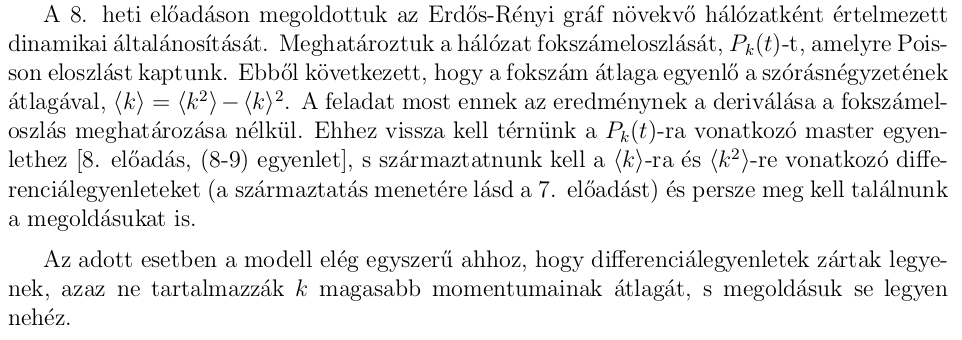
\includegraphics[width=1\textwidth]{elso.png}
	\end{center}
\end{figure}




\begin{center}
\underline{Feladat megoldása.}
\end{center}
\hspace{5cm}

A megoldáshoz a $P_k(t)$ re felírt master egyenletből indulunk ki:

\begin{center}
	\begin{gather*}
	\frac{\partial}{\partial t}P_k = P_{k-1} - P_k \\
	\frac{\partial}{\partial t}P_0 = -P_0
	\end{gather*}
\end{center}

A két alábbi momentum érdekel minket:

\begin{center}
	\begin{gather*}
	\langle k \rangle = \sum_{k =0}^{\infty}k P_k(t) \\
	\langle k^2 \rangle = \sum_{k =0}^{\infty}k^2 P_k(t)
	\end{gather*}
\end{center}

Első lépésben deriváljuk le $\langle k \rangle$-t, ahol most $k = 1$-gyel kezdődik:

\begin{center}
	\begin{gather*}
	\langle \frac{\partial}{\partial t} k \rangle = \sum_{k =0}^{\infty}k \frac{\partial}{\partial t}P_k(t) = \sum_{k = 1}^{\infty}kP_{k-1}(t) - \sum_{k = 1}^{\infty}kP_k(t).
	\end{gather*}
\end{center}

Átalakítom az egyenletet az alábbi egyenletek alapján:

\begin{center}
	\begin{gather*}
	\sum_{k = 1}^{\infty}kP_{k-1}(t) = \langle k \rangle +1 \\
	\sum_k P_k = 1. 
	\end{gather*}
\end{center}

Így az egyenletünk, ha mindent visszaírok, az alábbi egyenletet kapok:

\begin{center}
	\begin{equation}
		\langle \frac{\partial}{\partial t}k \rangle = \langle k \rangle + 1 - \langle k \rangle = 1. 
	\end{equation}
\end{center}

Majd a végeredményért elvégzem az integrálást:

\begin{center}
	\begin{equation}
	\langle k \rangle = t. 
	\end{equation}
\end{center}

Következő lépésben $\langle \frac{\partial}{\partial t}k^2 \rangle$ -t határozzuk meg:
\begin{center}
	\begin{gather}
	\langle \frac{\partial}{\partial t}k^2 \rangle = \sum_{k = 1}^{\infty} k^2 \frac{\partial}{\partial t}P_k(t) = \sum_{k = 1}^{\infty} k^2 P_{k-1}(t) - \sum_{k = 1}^{\infty} k^2 P_k(t),
	\end{gather}
\end{center}

ahol a második tagot felismerjük, hogy $\langle k^2\rangle$, a többit pedig átalakítom:

\begin{center}
	\begin{gather*}
	\sum_{k = 1}^{\infty}k^2 P_{k-1}(t) = \sum_{k = 1}^{\infty}(k-1)^2 P_{k-1}(t) + \sum_{k = 1}^{\infty}(2k-1)^2 P_{k-1}(t) =\\
	= \sum_{k = 1}^{\infty}k^2 P_{k-1}(t) + 2\sum_{k = 1}^{\infty}(k-1)^2 P_{k-1}(t) + \sum_{k = 1}^{\infty} P_{k-1}(t) = \\
	=\langle k^2 \rangle + 2\langle k\rangle +1.
	\end{gather*}
\end{center}

Ha mindent visszaírok és átrendezek:

\begin{center}
	\begin{equation}
	\langle \frac{\partial}{\partial t}k^2\rangle = 2 \langle k \rangle + 1.
	\end{equation}
\end{center}

Ebbe visszaírva $\langle k \rangle$-ra kapott értéket és kiintegrálom:

\begin{center}
	\begin{equation}
	\langle k^2 \rangle = t^2 + t.
	\end{equation}
\end{center}

Ha a kapott eredményeket beírom a feltett kérdésben szereplő egyenletbe, akkor megkapjuk a keresett értéket:

\begin{center}
	\begin{equation}
	t = \langle k \rangle = \langle k^2 \rangle - \langle k \rangle^2 = t^2 + t - t^2 = t.
	\end{equation}
\end{center}


\clearpage
%1
\section{feladat}

\begin{center}
	\underline{Feladat leírás.}
\end{center}

\begin{figure}[h!]
	\begin{center}
		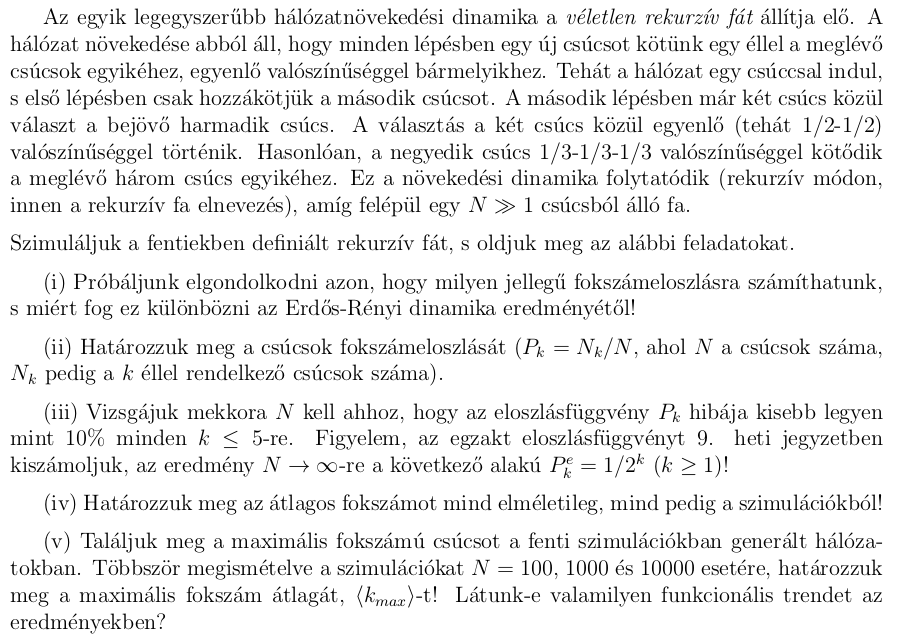
\includegraphics[width=1\textwidth]{masodik.png}
	\end{center}
\end{figure}

\clearpage
\begin{center}
	\underline{Feladat megoldása.}
\end{center}
\hspace{5cm}


\textit{(i)}\newline
Az Erdős-Rényi gráfban végig konstans a csúcsok száma, emiatt a mi esetünkben $\frac{1}{2^k}$ féle eloszlás alakul ki, míg az Erdős-Rényi gráfnál Gauss-eloszlás.\\
Valamint a mi esetünkben folyton növeljük a csúcsok számát.

A szimulációs feladatot most is \textit{python} programnyelven oldottam meg. Első lépésben létrehoztam N változót a lépések számát, amit majd változtatok a különböző lépésszámokra. Valamint a csúcsoknak és a fokszámoknak hoztam létre a tömböket és feltöltöttem a csúcsok tömbjét 1-től N-ig egyesével egész számokkal.
\newline
\rule{\textwidth}{0.1pt}
\begin{lstlisting}
%pylab inline
N = 10000

csucsok = numpy.zeros(N)
fokszamok = numpy.zeros(N)
for i in range (0,N):
	csucsok[i] = i+1
\end{lstlisting}
\rule{\textwidth}{0.1pt}

Az első és második csúcsot rögtön beállítom, hiszen azokat egyértelmű, hogy melyikhez tudjuk kötni őket.
\newline
\rule{\textwidth}{0.1pt}
\begin{lstlisting}
fokszamok[0] = 1
fokszamok[1] = 1
\end{lstlisting}
\rule{\textwidth}{0.1pt}

Majd betettem az új csúcsokat a hálózatba 2-től, N-ig. Fontos, hogy mikor beteszem az új csúcsot, akkor egy random csúcsot választok ki és ahhoz kötöm.
\newline
\rule{\textwidth}{0.1pt}
\begin{lstlisting}
for i in range (2,N):
	random_kivalasztott_csucs = randint(0,i)
	fokszamok[random_kivalasztott_csucs] += 1
	fokszamok[i] += 1
\end{lstlisting}
\rule{\textwidth}{0.1pt}

\clearpage
Majd kigyűjtöttem a fokszámokat és azok előfordulásának számát.\newline
\rule{\textwidth}{0.1pt}
\begin{lstlisting}
fokszameloszlas = []
fokszamokfajtaja = []
for i in range (0,N):
	if fokszamok[i] not in fokszamokfajtaja:
		fokszamokfajtaja.append(fokszamok[i])
		fokszameloszlas.append(1)
	if fokszamok[i] in fokszamokfajtaja:
		fokszameloszlas[fokszamokfajtaja.index(fokszamok[i])] += 1
\end{lstlisting}
\rule{\textwidth}{0.1pt}

Viszont sorrendbe kellett rendeznem a fokszámokat és a hozzá tartozó gyakoriságukat, mert az első kigyűjtés nem így hajtottam végre.\newline
\rule{\textwidth}{0.1pt}
\begin{lstlisting}
rendezett_fokszameloszlas = []
rendezett_fokszamokfajtaja = []
for i in range(1,len(fokszamokfajtaja)+1):
	for j in range(0,len(fokszamokfajtaja)):
		if fokszamokfajtaja[j] == i:
			rendezett_fokszamokfajtaja.append(i)
			rendezett_fokszameloszlas.append(fokszameloszlas[j])
\end{lstlisting}
\rule{\textwidth}{0.1pt}
\textit{(ii)}\\
Majd elkészítettem az eloszlásfüggvényt, mely: $P_k = \frac{N_k}{N}$, ahol $N_k$ a fokszámok gyakorisága, $N$ pedig az összes csúcsszám.\newline
\rule{\textwidth}{0.1pt}
\begin{lstlisting}
rendezett_fokszameloszlas = numpy.array(rendezett_fokszameloszlas)
rendezett_fokszamokfajtaja = numpy.array(rendezett_fokszamokfajtaja)
eloszlasfuggveny = rendezett_fokszameloszlas / N
\end{lstlisting}
\rule{\textwidth}{0.1pt}

Az előadáson levezetett érték stacionárius esetben $P_k^{stac} = \frac{1}{2^k}$, amit számoltam a programmal is és ábrázoltam is n = 10000.\newline
\rule{\textwidth}{0.1pt}
\begin{lstlisting}
def analitikus_mo(k):
	return 1/2**k
\end{lstlisting}
\rule{\textwidth}{0.1pt}

\begin{figure}[h!]
	\begin{center}
		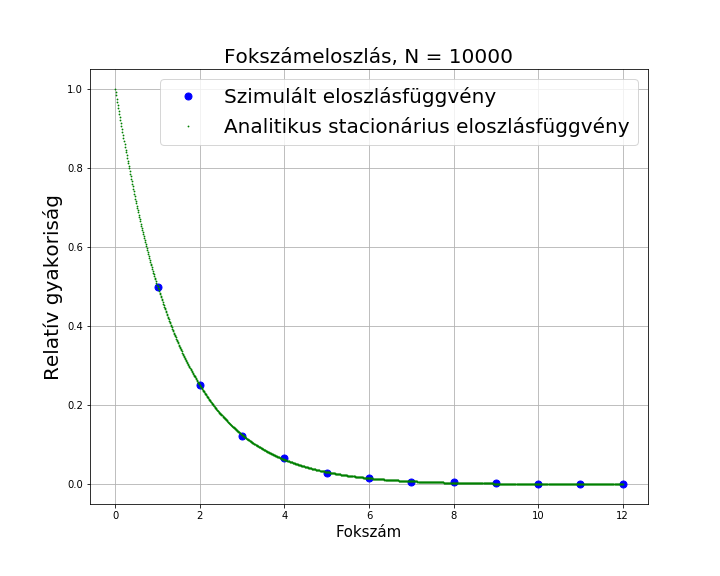
\includegraphics[width=0.8\textwidth]{fokszameloszlas.png}
	\end{center}
\caption{Szimulált és analitikus fokszámeloszlás példa, N = 10000 esetében.}
\end{figure}

\clearpage
\textit{(iii.)}\newline
A hiba meghatározásához a következő lépéseket végeztem:

\begin{itemize}
	\item a $k$ értékhez ismerjük a relatív gyakoriságot a szimulációból.
	\item az analitikus megoldást is kiszámolom a $k$ értékekhez.
	\item majd megnéztem, hogy hány százaléka a szimulált érték az analitikusnak.
	\item megállapítom, hogy hibahatáron belül van-e az érték.
\end{itemize}


A vizsgálat közben, mindig kiírattam, hogy melyik $k$ érték esetén van nagyobb, mint $10\%$, és így tudtam, hogy mennyit kell változtatnom  $N$ értékét. 
\newline
\rule{\textwidth}{0.1pt}
\begin{lstlisting}
arany = numpy.zeros(10)
if(eloszlasfuggveny.shape[0] < 10):
	meddig = eloszlasfuggveny.shape[0]
if(eloszlasfuggveny.shape[0] >= 10):
	meddig = 10
for k in range(0,meddig):
	arany[k] = eloszlasfuggveny[k] / analitikus_mo(k+1) * 100
	if(arany[k] < 90 or arany[k] > 110):
		print("k=" + str(k+1) +
		" eseten az elteres : " +
		str(abs(arany[k]-100)) + "%")
\end{lstlisting}
\rule{\textwidth}{0.1pt}

$N$ értékét 100-tól növeltem folyamatosan és úgy találtam, hogy mikor elértem a 200000 es $N$ számot, akkor már teljesült a $10\%$ alatti hibahatár\textit{(200000 felett is)}.

\clearpage
\textit{(iv)}\newline
Az átlagos fokszámot a szimuláció alapján, úgy kaptam meg, hogy kiátlagoltam a fokszámokat.
\newline
\rule{\textwidth}{0.1pt}
\begin{lstlisting}
atlagfokszam = 0
for i in range (0,shape(rendezett_fokszamokfajtaja)[0]):
	atlagfokszam += rendezett_fokszamokfajtaja[i] * rendezett_fokszameloszlas[i]
atlagfokszam = atlagfokszam / N
print("Atlagos fokszam szimulaciobol: " + str(atlagfokszam))
\end{lstlisting}
\rule{\textwidth}{0.1pt}


Hogy meg tudjam adni az átlagos fokszámot hibával együtt, lefuttattam a szimulációt különböző $N$-ekre, majd kiátlagoltam.\\
Az átlag hibája:

\begin{center}
	\begin{equation}
	\sigma^2 = \frac{1}{n}\sum_{i = 1}^{n}\left( x_i - \langle x\rangle \right)^2 \rightarrowtail \sigma = \sqrt{\sigma^2}.
	\end{equation}
\end{center}

\begin{table}[h!]
\begin{center}
\begin{tabular}{||c|c||}
	\hline
	N & $\langle k \rangle$ átlagos fokszám \\  \hline
	200000 & 2.000845 \\	\hline
	300000 & 2.000415 \\	\hline
	500000 & 2.000376 \\	\hline
	1000000 & 2.000169 \\	\hline
	10000000 & 2.0000225 \\	\hline
	Átlag hibával & 2.0003655 $\pm$ 0.0002788 \\  \hline
\end{tabular}
\caption{Átlagos fokszámhoz különböző N esetekre mérések, majd az átlagos fokszám hibával.}
\end{center}
\end{table}

A következő lépésben elméleti úton számolom ki $\langle k \rangle$ értékét.

\begin{center}
	\begin{equation}
	\sum_{k = 0}^{\infty} \frac{k}{2^k} = \sum_{k = 0}^{\infty} k\left( \frac{1}{2}\right)^k
	\end{equation}
\end{center}

Valamint a végtelen mértani sorról tudjuk azt:
\begin{center}
	\begin{equation}
	\sum_{k = 0}^{\infty} q^k = \frac{1}{1 - q},\ \ ha |q|<1, 
	\end{equation}
	\label{kell}
\end{center}

majd deriválom mindkét oldalt:

\begin{center}
	\begin{equation}
	\sum_{k = 0}^{\infty} k \cdot q^{k-1} = \frac{1}{(1 - q)^2}, 
	\end{equation}
\end{center}

majd átindexeljük:

\begin{center}
	\begin{equation}
	\sum_{k = 0}^{\infty} (k+1) \cdot q^{k} =  \frac{1}{(1 - q)^2}, 
	\end{equation}
	\label{kell2}
\end{center}

még egy kicsit alakítunk rajta:
\begin{center}
	\begin{equation}
	\sum_{k = 0}^{\infty} (k+1) \cdot q^{k} =  \sum_{k = 0}^{\infty} kq^k + \sum_{k = 0}^{\infty}q^k, 
	\end{equation}
	\label{kell3}
\end{center}


Felhasználom az előző összefüggéseket(\ref{kell}, \ref{kell2}):

\begin{center}
	\begin{equation}
	\sum_{k = 0}^{\infty} kk^q  =  \frac{1}{(1 - q)^2} - \frac{1}{1 - q} = \frac{q}{(1 - q)^2}. 
	\end{equation}
	\label{}
\end{center}

Most nekünk $k = 1/2$, tehát $\langle k \rangle$ átlagos fokszáma:

\begin{center}
	\begin{equation}
	\langle k \rangle = \frac{1/2}{(1-1/2)^2} = 2.
	\end{equation}
	\label{}
\end{center}

Tehát visszakaptam az előadáson kiszámolt megoldást, valamint szimulálva is ezt az értéket kaptam.\\
\clearpage
\textit{v.}\newline

Maximális fokszámot az alábbi kóddal kaptam meg:
\newline
\rule{\textwidth}{0.1pt}
\begin{lstlisting}
index = where(fokszamok == max(fokszamok))
print("Az ennyiedik csucs(ok)nak van maximalis fokszama:"
+ str(csucsok[index[0]]) +
 " ami ekkora fokszamu: " + str(max(fokszamok)))
\end{lstlisting}
\rule{\textwidth}{0.1pt}

A számolás eredményeit az alábbi táblázatok tartalmazzák:

\begin{table}[ht!]
	\begin{center}
		\begin{tabular}{||c|c||}
			\hline
			N & $\langle k_{max} \rangle$ maximális fokszám \\  \hline
			100 & 8 \\	\hline
100 & 8 \\	\hline
100 & 9\\	\hline
100 & 8\\	\hline
100 & 7\\	\hline
100 & 6\\	\hline
100 & 6\\	\hline
100 & 6\\	\hline
100 & 9\\	\hline
100 & 9\\	\hline
			Átlag hibával & 7.6 $\pm$ 1.2\\  \hline
		\end{tabular}
		\caption{$\langle k_{max} \rangle$ fokszámhoz különböző N = 100 esetekre.}
	\end{center}
\end{table}


\begin{table}[ht!]
	\begin{center}
		\begin{tabular}{||c|c||}
			\hline
			N & $\langle k_{max} \rangle$ maximális fokszám \\  \hline
			1000 & 10 \\	\hline
			1000 & 12 \\	\hline
			1000 & 11\\	\hline
			1000 & 10\\	\hline
			1000 & 11\\	\hline
			1000 &11\\	\hline
			1000 & 11\\	\hline
			1000 & 10\\	\hline
			1000 & 10\\	\hline
			1000 & 13\\	\hline
			Átlag hibával & 10.9 $\pm$ 0.943\\  \hline
		\end{tabular}
		\caption{$\langle k_{max} \rangle$ fokszámhoz különböző N = 1000 esetekre.}
	\end{center}
\end{table}


\begin{table}[ht!]
	\begin{center}
		\begin{tabular}{||c|c||}
			\hline
			N & $\langle k_{max} \rangle$ maximális fokszám \\  \hline
			10000 & 13 \\	\hline
			10000 & 14 \\	\hline
			10000 & 14\\	\hline
			10000 & 13\\	\hline
			10000 & 15\\	\hline
			10000 & 15\\	\hline
			10000 & 15\\	\hline
			10000 & 14\\	\hline
			10000& 16\\	\hline
			10000 & 13\\	\hline
			Átlag hibával & 14.2 $\pm$ 0.979\\  \hline
		\end{tabular}
		\caption{$\langle k_{max} \rangle$ fokszámhoz különböző N = 10000 esetekre.}
	\end{center}
\end{table}

\begin{figure}[h!]
	\begin{center}
		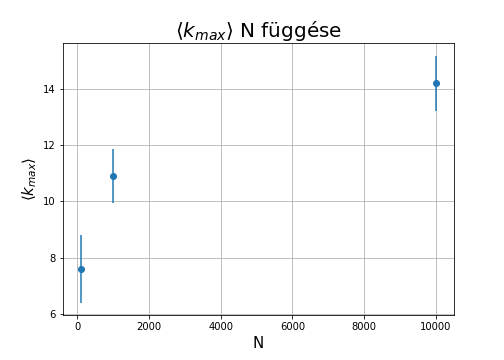
\includegraphics[width=0.8\textwidth]{kmax.png}
	\end{center}
	\caption{$\langle k_{max} \rangle$ maximális fokszám N függése.}
\end{figure}



\end{document}